\chapter{Implementacja programowa oraz sprzętowa wybranej architektury sieci}
\label{cha:Implementacja}
% Opis oraz omówienie implementacji zarówno programowej jak i~sprzętowej.

Opracowanie odpowiedniej architektury sieci oprócz rozważań teoretycznych, wymagało również wykonania szeregu eksperymentów obliczeniowych.
Ponadto konieczna była implementacja sprzętowa modelu celem akceleracji obliczeń zaprojektowanej architektury na wybranej platformie obliczeniowej.

\section{Implementacja programowa}

Implementacja programowa została zrealizowana w~ramach framework'a \emph{PyTorch} \cite{pytorch}.
Wykorzystano również bibliotekę \emph{Brevitas} \cite{brevitas} do realizacji odpowiedniej metody kwantyzacji.
Metodyka implementacji kwantyzacji opiera się o~klasę \emph{ExtendedInjector}.
Pozwala ona na ``wstawienie'' operacji kwantyzacji wag bezpośrednio przed zastosowaniem ich w~obliczeniach.
Ponadto biblioteka rozszerza predefiniowane w~\emph{PyTorch} warstwy o~operacje kwantyzacji. 
W wersji kwantyzowanej dostępne są m.in. warstwa konwolucji, \emph{Max Pooling} czy funkcja $ReLU$.
Kwantyzowana warstwa normalizacji została zdefiniowana jako przekształcenie afiniczne bez aproksymacji średniej i~wariancji.
Wymagało to implementacji własnej warstwy dokonującej wyboru pomiędzy warstwą zmiennoprzecinkową oraz jej wersją kwantyzowaną.
Augmentacja danych została zrealizowana w~oparciu o~bibliotekę \emph{OpenCV} \cite{opencv}.
Obliczenia były wykonywane na platformie \emph{GoogleColab} \cite{colab} z~wykorzystaniem \emph{GPU}.
Ze względu, iż dzienny czas użytkowania usługi jest ograniczony wymagane było przechowywanie stanu procesu ucznia w~plikach zapisywanych poprzez usługę \emph{GoogleDrive}.


Dla celu testowania wyników implementacji sprzętowej poszczególnych warstw został zaimplementowany dodatkowy model programowy (dwóch typów warstw). 
Wykorzystywał on obliczenia całkowitoliczbowe do wykonania operacji konwolucji \emph{DW} oraz \emph{PW}.
Ponadto zaimplementowano także konwersję wag zmiennoprzecinkowych do stałoprzecinkowych wymaganych do inicjalizacji pamięci ROM akceleratorów opisanych w~dalszej części.

\section{Implementacja sprzętowa}

Wstępnie planowano implementacje sprzętową z~wykorzystaniem narzędzia \emph{FINN} \ref{ch:tools}.
Jednakże ze względu na braki w~dokumentacji (np. implementacja własnej metody kwantyzacji w~\emph{Brevitas}), a~także brak możliwości akceleracji warstwy \emph{BN} (przynajmniej bezpośrednio) zdecydowano się na implementację własną.
Początkowo w~języku wysokopoziomowym \emph{HLS}, lecz ostatecznie w~języku opisu sprzętu \emph{System Verilog}
%, uzyskując w ten sposób pełną kontrolę sposobem implementacji
.
Akceleracja całej sieci stanowi architekturę potokową gruboziarnistą (ang. \emph{coarse grained}).
Schemat przedstawiono na rysunku \ref{fig:LNACC}.
Na elementy wspomnianej architektury składają się:
\begin{description}
\item  bloki komunikacji - realizują wymianę danych z~\emph{DMA} (ang. \emph{Direct Memory Access}) \cite{dma} poprzez magistralą \emph{AXI4-Stream} \cite{axis}. 
Blok \emph{AXIS RECEIVER} odbiera i przekształca strumień danych do postaci wymaganej na dalszym etapie. Wysyłanie danych odbywa się poprzez blok \emph{AXIS SENDER}.
\item \emph{IL} (ang. \emph{Input Layer}) - warstwa wejściowa zmiana formatu danych wejściowych.
\item \emph{ROM}(ang. \emph{Read-Only Memory}) - przechowywanie wag poszczególnych warstw.
\item \emph{RAM})(ang. \emph{Random Access Memory}) - przechowywanie danych wejściowych oraz rezultatów poszczególnych akceleratorów.
\item multipleksery - zarządzanie dostępem do pamięci.
\item \emph{DW, PW, BN, MP, B} - bloki akceleratorów warstw w zadanych konfiguracjach.
Poszczególne akceleratory pogrupowane są po 3 w~bloku. 
Na jeden blok przypisane są dwa bloki pamięci RAM, w~tym jeden z~dostępem  multipleksowanym.
Ma to na celu ograniczenie wymaganej pamięci, kosztem zmniejszenia przepustowości. 
\item \emph{SSR} - rejestr szeregowo-równoległy (ang. \emph{Serial-Parallel Register}) realizuje odbiór danych z ostatniej warstwy.
\item \emph{LN\_CU} (ang. \emph{LittleNet Control Unit}) -  logika sterująca procesem akceleracji.
\end{description}

% Na elementy wspomnianej architektury składają się bloki komunikacji zewnętrznej, pamięci RAM oraz ROM, multipleksery dostępu do pamięci, akceleratory poszczególnych warstw oraz logika sterująca (\emph{LN\_CU}, ang. \emph{LittleNet Control Unit}).
% Wykorzystywana jest tutaj komunikacja z~wykorzystaniem protokołu \emph{AXI4-Stream} \cite{axis} do komunikacji z~\emph{DMA} (ang. \emph{Direct Memory Access}) \cite{dma}.
% Wymiana danych odbywa się za pośrednictwem  modułów \emph{AXIS RECEIVER} do odbioru oraz \emph{AXIS SENDER} do wysyłania danych zgromadzonych w~rejestrze \emph{SPR} (ang. \emph{Serial-Parallel Register}).

Proces akceleracji odbywa się według schematu prezentowanego w~tabeli \ref{tab:LNACC}.
Zostało to zrealizowane w postaci maszyny stanów.
W danym stanie 0-3 aktywne są akceleratory 0-2 z bloków 0-5, dla których występuje wartość 1.
W tabeli \ref{tab:LNACC} oznaczono również typy każdego akceleratora.
Pozwala to uzyskać ciąg operacji przetwarzania danych tożsamy z architekturą sieci. 
W jednej chwili są aktywne akceleratory co czwartej warstwy.
Jest to wymagane, aby udzielić dostępu do wybranych bloków pamięci kilku akceleratorom.

\begin{figure}
    \centering
    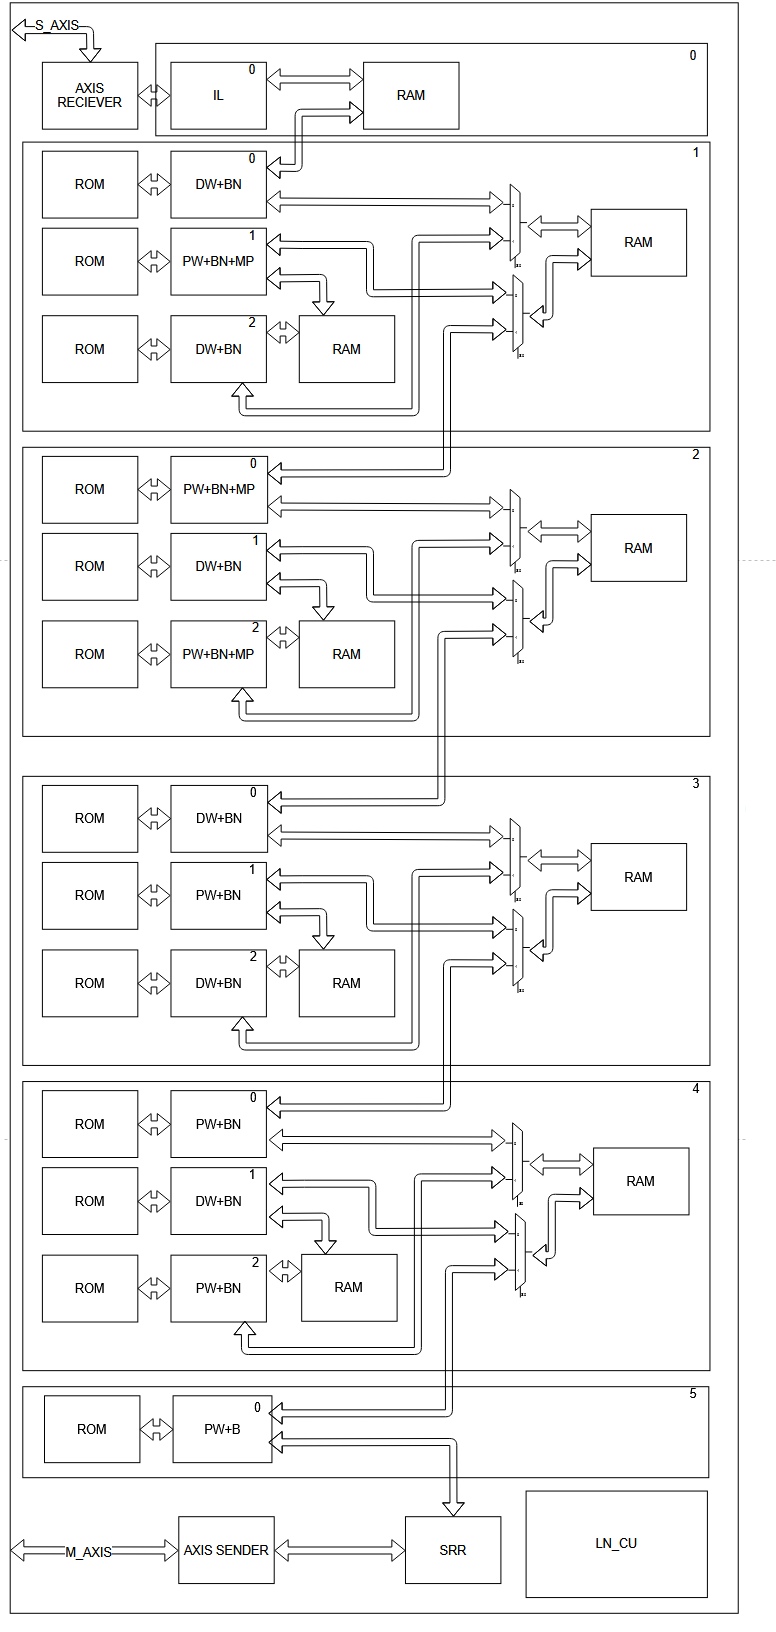
\includegraphics[height=0.9\textheight]{images/LNACC.png}
    \caption{Schemat akceleracji architektury \emph{LittleNet}. Uwzględniono jedynie najistotniejsze elementy.}
    \label{fig:LNACC}
\end{figure}
\begin{table}
    \centering
    \caption{Schemat aktywacji akceleratorów zrealizowany jako maszyna stanów.}
    \label{tab:LNACC}
    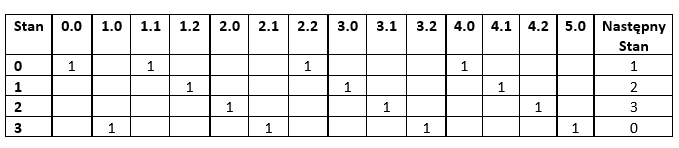
\includegraphics[width=0.9\textwidth]{images/acc_activ.png}
\end{table}

Wyróżniono 3 typy akceleratorów (dostępnych w~kilku konfiguracjach):
\begin{description}
\item warstwa wejściowa (IL),
\item warstwa \emph{depthwise} (DW),
\item warstwa \emph{pointwise} (PW).
\end{description}

Akceleratory warstw \emph{PW} pozwalają na równoległe wykonanie operacji.
Jednakże wymagany jest zapis do jednej pamięci w sposób szeregowy.
Do tego celu  wykorzystywany jest moduł \emph{MWU} (ang. \emph{Memory Writer Unit}) przedstawiony na rysunku \ref{fig:mwu}.
Wykonuje on operacje analogiczne do rejestru równoległo-szeregowego (o $P$ kanałach wejściowych).
Równoległe kanały wejściowe $CH\_i$ $P$ są odpowiednio opóźniane. 
Każdy kanał $CH\_{i}$ przechodzi przez linię opóźniającą \emph{D} o~latencji równej indeksowi sygnału $i$.
Do każdego kanału przypisany jest licznik adresu $CHD\_i$.
W przypadku, gdy opóźniona wartość kanału jest uznawana za ważną (ang. \emph{valid}) następuje inkrementacja adresu.
Wszystkie opóźnione kanały są multipleksowane przez moduł \emph{MUX}, wybierając kolejne kanały.
Wartość wybranego kanału wraz z opowiadającym adresem stanowią interfejs pamięci docelowej.
Ponadto dodatkowa logika sterująca została przedstawiona poprzez blok \emph{MW\_CU}(ang. \emph{Memory Writer Control Unit}).
\begin{figure}
    \centering
    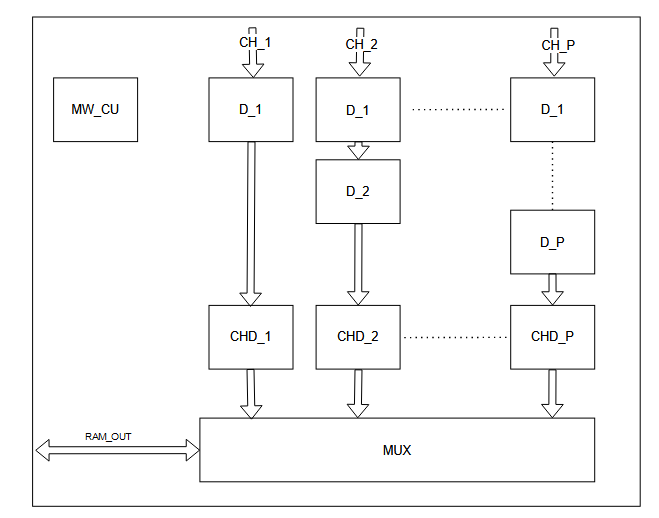
\includegraphics[width=0.8\linewidth]{images/MWU.png}
    \caption{\emph{MWU} -- schemat generowania adresu dla przetwarzania wielokanałowego.}
    \label{fig:mwu}
\end{figure}

\subsection{Warstwa wejsciowa}

Warstwa wejściowa \emph{IL} (ang. \emph{Input Layer}) realizuje zadanie zmiany formatu danych.
Schemat akceleratora został przedstawiony na rysunku \ref{fig:il}.
Dane wejściowe otrzymywane są w~notacji \emph{H-W-CH} (ang \emph{Height-Width-Channel}).
Na dalszym etapie przetwarzania wymagany jest format \emph{CH-H-W}.
Realizowane jest to poprzez buforowanie 3 kolejnych 32 bitowych pakietów danych w~rejestrze szeregowo-równoległym \emph{SPR}.
Zgromadzone dane są rozdzielane na poszczególne kanały \emph{R-G-B} (ang. \emph{Red-Green-Blue}) składając się na 32 bitowe pakiety po jednym na każdy kanał.
Uzyskany podział jest zapisywany do pamięci poprzez moduł \emph{MWU} dla 3 kanałów.
\begin{figure}
    \centering
    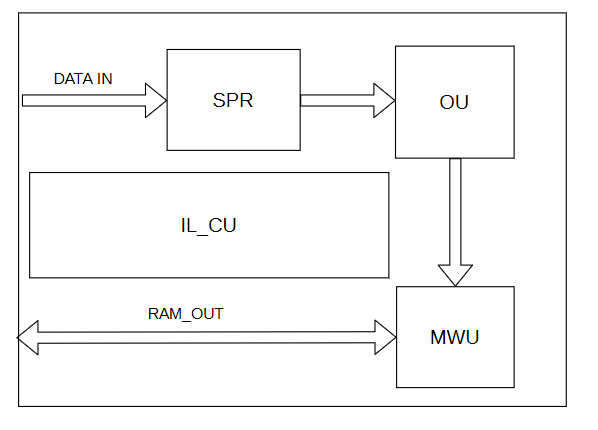
\includegraphics[width=0.8\linewidth]{images/ILACC.png}
    \caption{Schemat warstwy wejściowej \emph{IL}.}
    \label{fig:il}
\end{figure}

\subsection{Warstwa \emph{depthwise (DW)}}

Akceleracja konwolucji \emph{DW} jest realizowana razem z~warstwą normalizującą.
Na rysunku \ref{fig:dwacc} przedstawiono schemat akceleratora \emph{DW}.
Obliczenia wykonywane są w~architekturze potokowej drobnoziarnistej (ang. \emph{fine grained}). 
W tym celu moduł \emph{SWU} (ang. \emph{Sliding Window Unit}) generuje strumień danych wraz z~odpowiednimi opóźnieniami tak, aby uzyskać kontekst okna przesuwnego o~wymiarach 3x3.
Wykonanie operacji konwolucji wymaga wcześniejszego (przed rozpoczęciem strumieniowania każdego kanału) wczytania wag maski konwolucji.
Operację tę wykonuje moduł \emph{WSL} (ang. \textit{Weights Loading Unit}).
Sama operacja iloczynu skalarnego wektora wag i~kontekstu jest wykonywana przez \emph{DW\_PU} (ang. \emph{DepthWise Processing Unit}) przedstawiony na schemacie \ref{fig:dwpu}.
Wykorzystano tutaj możliwość kaskadowego połączenia kolejnych 9 \emph{DSP}. 
Dostępna jest konfiguracja wykorzystująca składową bias konwolucji (\emph{B}) oraz normalizację poprzez przekształcenie afiniczne (\emph{BN}).
Wynik konwolucji oraz normalizacji jest ograniczany (\emph{LIMIT}) do wartości wynikających z~wybranej notacji stałoprzecinkowej, czy też zastosowania funkcji $ReLU$.

Uzyskany rezultat jest zapisywany pod adresem wyznaczonym przez \emph{MWU}.
Sterowanie procesem akceleracji odbywa się poprzez logikę reprezentowaną przez \emph{DW\_CU} (ang. \emph{DepthWise Control Unit}).
Wykonanie wielokrotnej konwolucji \emph{DW} odbywa się poprzez wielokrotne (cykliczne) generowanie strumienia danych wejściowych przez \emph{SWU}.
\begin{figure}
    \centering
    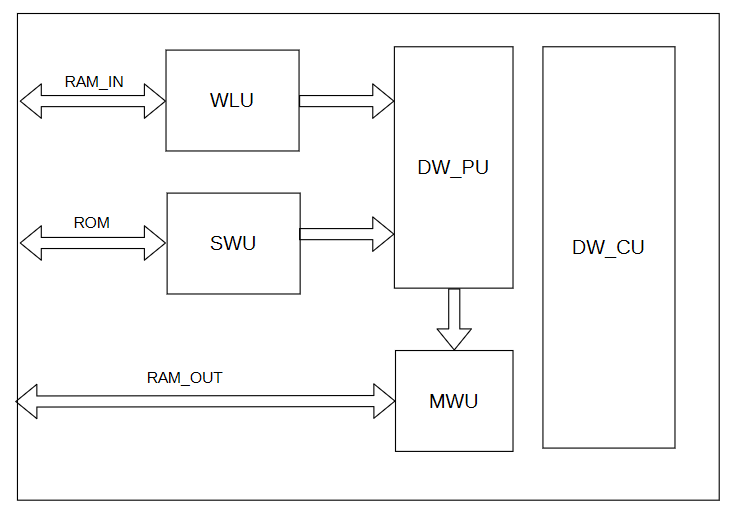
\includegraphics[width=0.9\linewidth]{images/DWACC.png}
    \caption{Schemat akceleratora \emph{DW} dostępnego w~wielu konfiguracjach.}
    \label{fig:dwacc}
\end{figure}
\begin{figure}
    \centering
    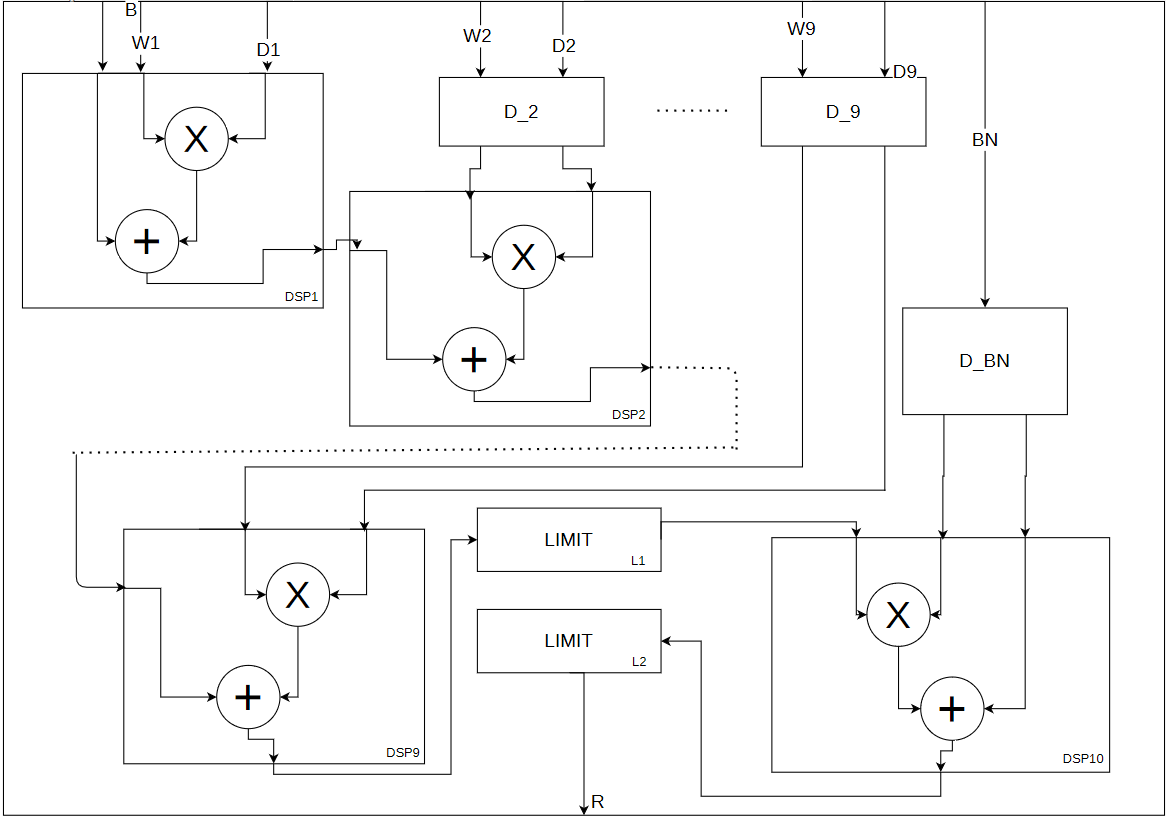
\includegraphics[width=0.9\linewidth]{images/DW_PU.png}
    \caption{Schemat \emph{DW\_PU} -- kaskadowe połączenie \emph{DSP}.
    Bloki \emph{DSP10+L2} są opcjonalne zależnie od konfiguracji.}
    \label{fig:dwpu}
\end{figure}

\subsection{Warstwa \emph{pointwise (PW)}}

Podobnie jak w~poprzednim przypadku akcelerator konwolucji \emph{PW} dostępny jest w~wielu konfiguracjach.
Schemat akceleratora \emph{PW} prezentuje rysunek \ref{fig:pwacc}.
Operacja konwolucji \emph{PW} nie wymaga gromadzenia otoczenia rozpatrywanego punktu, lecz iterowania po kolejnych kanałach wejściowych w~danym punkcie.
Jest to realizowane przez moduł \emph{PSU} (ang. \emph{Point Streamer Unit}).
Dla każdego kanału rozważanego punktu jest wymagana odpowiednia waga.
Ponadto identyczna sekwencja wag jest powtarzana dla następnych puntów.
W tym celu moduł \emph{CSU} (ang. \emph{Cyclic Streamer Unit}) generuje strumień w~sposób cykliczny.
Następuje wielokrotny odczyt z~kolejnych adresów zadanej puli adresowej definiowanej przez liczbę wag filtru. 
Przed rozpoczęciem generowania strumienia danych, odczytywane są wagi bias oraz przekształcenia afinicznego, które następnie są przechowaniem w~odpowiednich rejestrach.
Obliczenie konwolucji dla kolejnych punktów jest realizowane przez moduł \emph{PW\_PU} (ang. \emph{PointWise Processing Unit}) (rysunek \ref{fig:pwpu}).
Wykorzystuje się do tego celu operacje akumulacji z~mnożeniem.
Zakumulowana suma iloczynów jest (zależnie od konfiguracji) powiększana o~wartość bias.
Uzyskany rezultat zostaje ograniczony (identycznie jak w~konwolucji \emph{DW}).
W następnym kroku wykonywana jest operacja normalizacji wraz z~ponownym ograniczeniem wartości.

Następnym etapem przetwarzania jest (ewentualna) operacja \emph{Max Pooling}.
Do tego celu wykorzystuje się odpowiednie opóźnienia oraz porównywania wartości.
Uzyskany rezultat jest zapisywany pod adresem wyznaczanym przez moduł \emph{MWU}.
Opcjonalną funkcjonalnością (dla warstwy \emph{YOLOv3}) jest zastąpienie \emph{MWU} przez \emph{MFU} (ang. \emph{Max Finder Unit}) pozwalającego znaleźć punkt o~największej wartości (funkcja \emph{argmax}) wykrywalności obiektu, a~także zwrócić jego parametry (funkcja \emph{max}).
Ponadto istnieje możliwość zrównoleglenia obliczeń poprzez wykorzystanie $P$ modułów \emph{PW\_PU}. 
Wymaga to zastosowania pamięci ROM $P$-krotnie szerszej. 
Sterowanie poszczególnymi modułami jest zaimplementowane w bloku \emph{PW\_CU} (ang. \emph{PointWise Control Unit}).

\begin{figure}
    \centering
    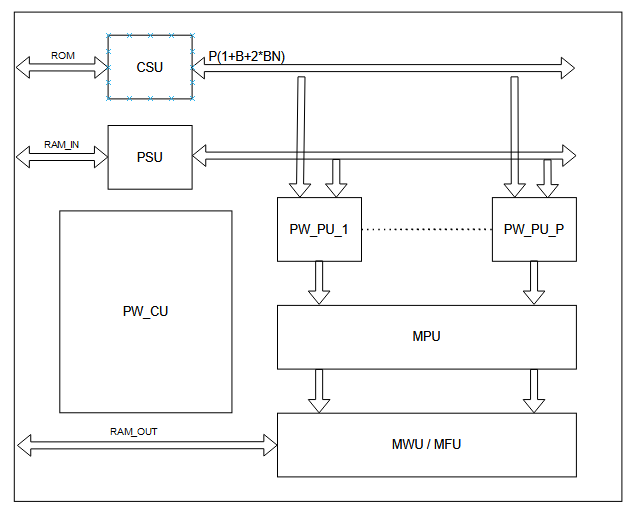
\includegraphics[width=0.9\linewidth]{images/PWACC.png}
    \caption{Schemat akceleratora \emph{PW} dostępnego w~wielu konfiguracjach.
    Opcjonalne są moduły \emph{MPU} oraz \emph{MWU} lub \emph{MFU}.}
    \label{fig:pwacc}
\end{figure}
\begin{figure}
    \centering
    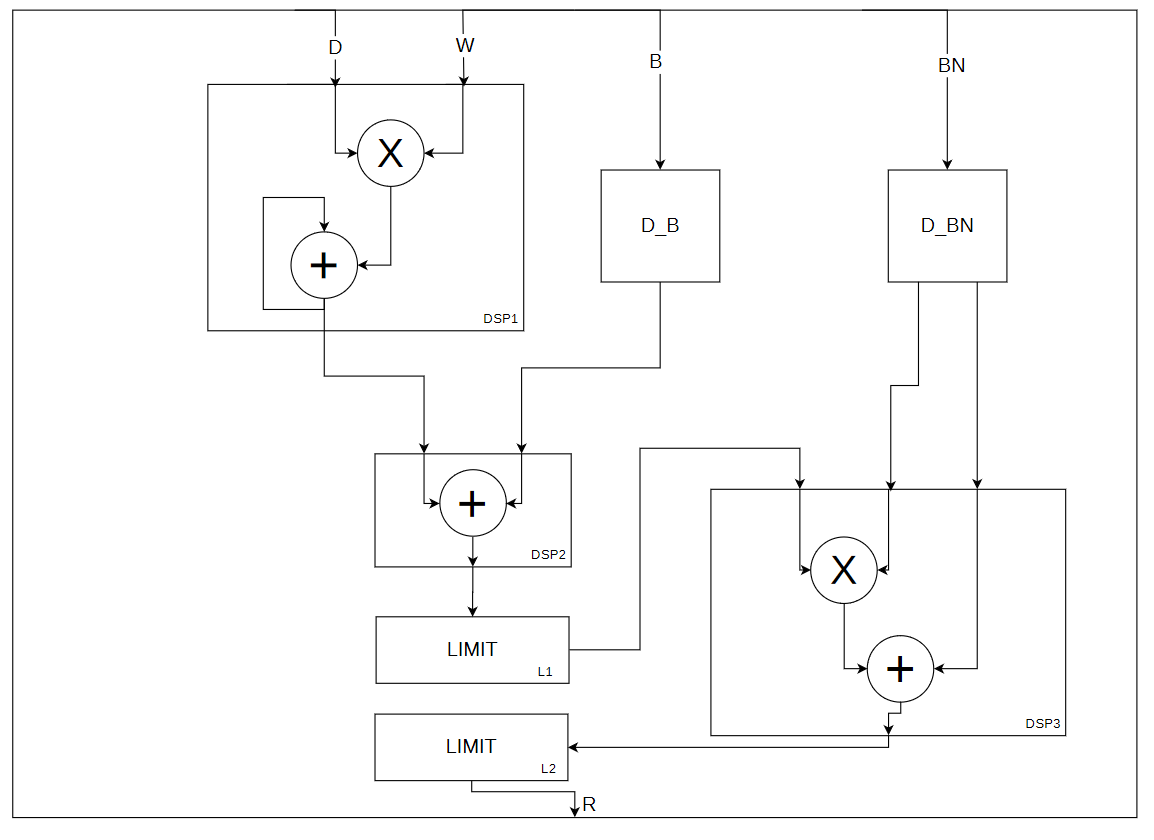
\includegraphics[width=0.8\linewidth]{images/PW_PU.png}
    \caption{Schemat \emph{PW\_PU} -- akumulacja z~mnożeniem realizowane przez \emph{DSP}. Bloki \emph{DSP2} oraz \emph{DSP3+L2} są opcjonalne i~zależne od konfiguracji.}
    \label{fig:pwpu}
\end{figure}

\subsection{Sterowanie akceleracją}

\label{ch:sterowanie}
Zaimplementowany akcelerator sieci \emph{LittleNet} został dołączony do schematu blokowego dostarczonego przez organizatorów konkursu.
Zmodyfikowany schemat przedstawiono na rysunku \ref{fig:vivado}. 
\begin{figure}
    \centering
    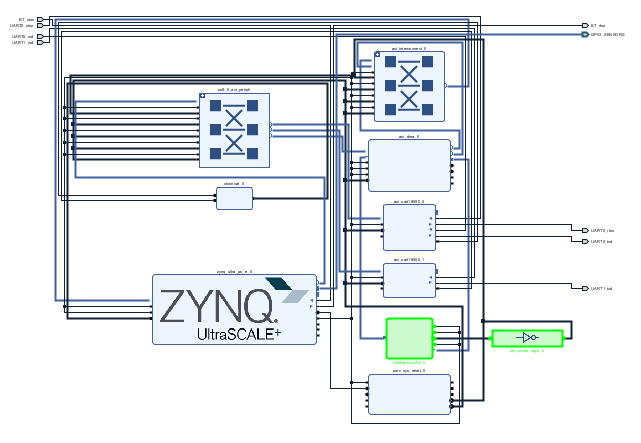
\includegraphics[width=0.9\linewidth]{images/vivado.png}
    \caption{Schemat blokowy w~środowisku \emph{Vivado 2019.1}. Zaznaczono dodane elementy -- akcelerator oraz negacja sygnału \emph{reset}.}
    \label{fig:vivado}
\end{figure}

Uzyskaną modyfikacją poddano syntezie, implementacji oraz wygenerowano plik \emph{bit} w~środowisku \emph{Vivado 2019.1} dostarczonym przez firmę \emph{Xilinx}.
Otrzymane rezultaty (pliki \emph{*.hwh} oraz \emph{*.bit}) umieszczono w~odpowiednio skonfigurowanym środowisku na platformie \emph{Avnet Ultra96 V2}.
Aplikacje sterującą zrealizowano w~postaci notatnika \emph{Jupyter}.
Konfiguracja logiki programowalnej oraz przesył danych do oraz z~akceleratora zostały zrealizowane z~użyciem biblioteki \emph{PYNQ}. 
Odczyt obrazów oraz przetwarzanie rezultatów zaimplementowano w~sposób równoległy do procesu akceleracji.
Analizując dokładniej schemat akceleracji można zauważyć, iż rezultat przetwarzania danego obrazu jest uzyskiwany po 4 cyklach przetwarzania.
Wymaga to odrzucenia początkowych rezultatów oraz wykonania dodatkowych cykli akceleracji, aby uzyskać poprawny wynik dla wszystkich obrazów wejściowych.


\section{Podsumowanie}
Przeprowadzony proces implementacji wymagał na początkowym etapie wyznaczenia modelu programowego. 
W tego celu wykorzystano biblioteką \emph{PyTorch} oraz \emph{Brevitas}.
Pierwszy etap wymagał wytrenowania modelu zmiennoprzecinkowego.
Uzyskany model zastał następnie poddany odpowiedniej kwantyzacji.
Zrealizowanie sprzętowej akceleracji wymagało opracowania sposobu implementacji poszczególnych warstw, jak i~całej sieci.
Wyszczególniono 3 typy akceleratorów: warstwa wejściowa,  \emph{DW} oraz \emph{PW}.
Pierwsza z~wymienionych dokonuje zmiany formatu danych wejściowych.
Pozostałe dwie warstwy realizuję odpowiednie konwolucje wraz z~normalizacją.
Warstwa \emph{PW} możliwa jest do konfiguracji realizującej operacje \emph{Max Pooling} czy też funkcji \emph{argmax} oraz \emph{max}. 
Możliwe jest także dodatkowe zrównoleglenie poprzez wykorzystanie większej liczby modułów \emph{PW\_PU}. 
Akceleracja całej sieci oparta jest o~architekturę potokową gruboziarnistą z~opóźnieniem 4 cykli przetwarzania.
Zastosowanie akceleratora do przetwarzania obrazów wymagało implementacji z~wykorzystaniem notatnika \emph{Jupyter} możliwego do modyfikacji w~trakcie ewaluacji. 












